\documentclass[12pt]{article}
\usepackage{url, graphicx, epstopdf, amsmath, esint}
\usepackage{physics}

% page layout
\setlength{\topmargin}{-0.25in}
\setlength{\textheight}{9.5in}
\setlength{\headheight}{0in}
\setlength{\headsep}{0in}
\setlength{\parindent}{1.1\baselineskip}
\addtolength{\oddsidemargin}{-0.75in}
\setlength{\marginparwidth}{2in}

% problem formatting
\newcommand{\problemname}{Problem}
\newcounter{problem}
\newcommand{\startproblem}{\paragraph{Problem~\theproblem:}\refstepcounter{problem}}

% words
\newcommand{\foreign}[1]{\textsl{#1}}
\newcommand{\vs}{\foreign{vs}}

% math
\renewcommand{\vec}[1]{\boldsymbol{#1}}
% \newcommand{\dd}{\mathrm{d}} % PROVIDED IN physics PACKAGE
\newcommand{\e}{\mathrm{e}}
% \newcommand{\cross}{\times} % PROVIDED IN physics PACKAGE
% \newcommand{\curl}{\vec{\nabla}\times} % PROVIDED IN physics PACKAGE

% primary units
\newcommand{\rad}{\mathrm{rad}}
\newcommand{\kg}{\mathrm{kg}}
\newcommand{\m}{\mathrm{m}}
\newcommand{\s}{\mathrm{s}}
\newcommand{\A}{\mathrm{A}}

% secondary units
\renewcommand{\deg}{\mathrm{deg}}
\newcommand{\km}{\mathrm{km}}
\newcommand{\cm}{\mathrm{cm}}
\newcommand{\mm}{\mathrm{mm}}
\newcommand{\mum}{\mathrm{\mu m}}
\newcommand{\nm}{\mathrm{nm}}
\newcommand{\ft}{\mathrm{ft}}
\newcommand{\mi}{\mathrm{mi}}
\newcommand{\AU}{\mathrm{AU}}
\newcommand{\ns}{\mathrm{ns}}
\newcommand{\h}{\mathrm{h}}
\newcommand{\yr}{\mathrm{yr}}
\newcommand{\N}{\mathrm{N}}
\newcommand{\J}{\mathrm{J}}
\newcommand{\eV}{\mathrm{eV}}
\newcommand{\MeV}{\mathrm{MeV}}
\newcommand{\W}{\mathrm{W}}
\newcommand{\Pa}{\mathrm{Pa}}
\newcommand{\C}{\mathrm{C}}
\newcommand{\V}{\mathrm{V}}
\newcommand{\ohm}{\mathrm{\Omega}}
\newcommand{\muF}{\mathrm{\mu F}}
\newcommand{\Hz}{\mathrm{Hz}}
\newcommand{\GHz}{\mathrm{GHz}}

% derived units
\newcommand{\mps}{\m\,\s^{-1}}
\newcommand{\mph}{\mi\,\h^{-1}}
\newcommand{\mpss}{\m\,\s^{-2}}
\newcommand{\radps}{\rad\,\s^{-1}}

% random stuff
\sloppy\sloppypar\raggedbottom\frenchspacing\thispagestyle{empty}

\begin{document}

\section*{NYU Physics 2---Problem Set 11}

Due Thursday 2020 April 30 before lecture.

\paragraph{Problem~\theproblem:}\refstepcounter{problem}%
A low-pass filter for voltage can be created as shown.
For any input AC voltage amplitude $V$,
the output voltage $V_{ab}$ will be a strong function of frequency $\omega$.
Set the resistance to $120\,\ohm$ and the capacitance to $100\,\muF$
and plot the ratio $|V_{ab}|/V$ as a function of
$\omega$ over the range $0<\omega<2000\,\radps$.
Label your plot with the value of the voltage ratio at $\omega\rightarrow 0$ and
with the frequency $\omega_{1/2}$ at which the voltage ratio is half of its
value at zero frequency. Write that latter label with a numerical value with proper
units.
\marginpar{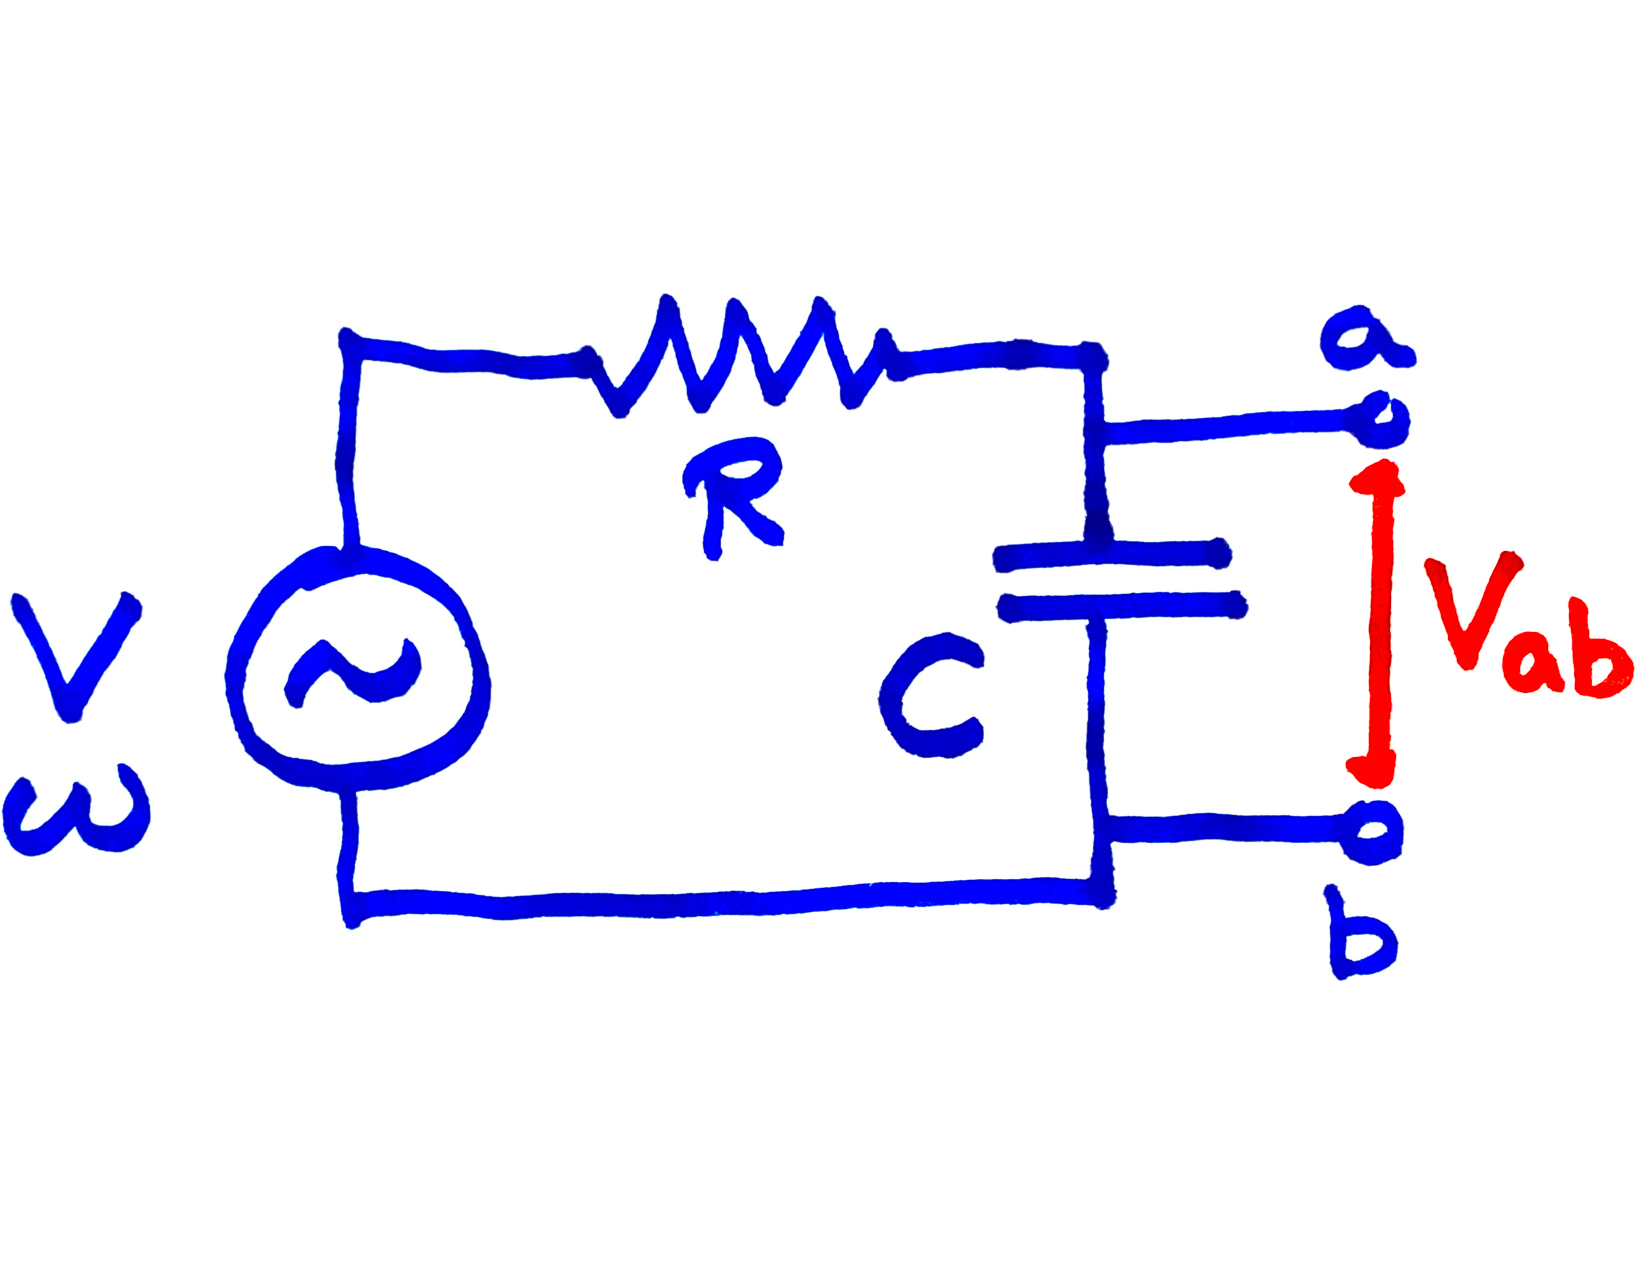
\includegraphics[width=\marginparwidth]{lowpass.pdf}}

Note that the voltage ratio $|V_{ab}|/V$ involves a magnitude because the
voltage amplitude $V_{ab}$ will be a complex number. This problem and the
next one will really make use of the complex impedance rules.

\paragraph{Problem~\theproblem:}\refstepcounter{problem}%
In Lecture we solved the problem of an AC circuit where the generator,
capacitor, resistor, and inductor are all in series.
Now solve the problem for the AC circuit where all four components are
in parallel with one another.
That is, what is the complex impedance $Z$ of $L, R, C$ all in parallel?
And what is the complex current amplitude $I$
and its magnitude $|I|$ given the AC input voltage
with amplitude $V$ and frequency $\omega$?

\paragraph{Problem~\theproblem:}\refstepcounter{problem}%
Imagine you have a long straight wire running along the $x$-axis.
Now imagine that centered at $x=0$ there is a parallel-plate capacitor
with circular plates of radius $a$, separated by a tiny gap $h\ll a$,
with the plates perpendicular to the wire.
Current $I$ is flowing in the $x$ direction, so the capacitor is charging.
Consider an Ampere's law loop of radius $r$ that is circular
and centered on the origin, and lying in the $y$--$z$ plane.
That is, the loop is centered in the gap between the plates of the capacitor.
Using the $\dd\vec{E}/\dd t$ term in Maxwell's equations,
compute the magnetic field magnitude $|\vec{B}|$ as a function of $r$ over
the range $0<r<3\,a$.
Plot your result $|\vec{B}|$ \foreign{vs} $r$, labeling the value at
$r=0$ and the maximum value.
Show that at $r>a$ you get for $|\vec{B}|$ what you would have gotten if you had just used
the $\mu_0\,I$ term instead of the $\dd\vec{E}/\dd t$ term.

\paragraph{Problem~\theproblem:}\refstepcounter{problem}%
Let's build a model of the fields inside a resistor.
Imagine you have a perfectly cylindrical resistor of length $\ell$ and
radius $a$, carrying total current $I$. If the total resistance is $R$,
then there is a voltage drop $V=I\,R$ down the length of the resistor. This
means that the resistor contains an electric field $\vec{E}$ inside it. What is
the magnitude $|\vec{E}|$ and direction of that field $E$?
Give your answer in terms of $R, \ell, I$.

Now that $\vec{E}$ field must be created by charges; where are those charges?
What charge densities must exist in this problem, and where? Imagine that
the ends of the resistor are conducting circular plates of radius $a$ and
the interior of the resistor is some kind of resistive material. Does it
make sense now that any resistor must also have capacitance? Roughly how
much charge $+Q, -Q$ must be on those plates?
Give your answer in terms of $R, \ell, a, I$.

In order to solve this problem, assume that the $\vec{E}$ field is entirely
contained inside the resistor. That's not true! But this problem is intended
to be conceptual not exact.

Now imagine (incorrectly, it also turns out) that the current is uniformly distributed
throughout the resistor. What is the current density $\vec{J}$ inside the
resistor (magnitude and direction). You might have to look up the definition
of current density in your textbook. The resistivity $\rho$ we encountered in a
previous Problem Set should be related to these by $\vec{E}=\rho\,\vec{J}$.
This is the ``differential form'' of Ohm's Law.
Check that this works out in terms of units.

Now, finally, what is the direction and magnitude of the magnetic field $\vec{B}$
at the surface of the resistor? In the final week of class, the quantity
$\vec{E}\times\vec{B}$ will become important. Which way does that vector point in
this case? If you want to read ahead, look up ``Poynting flux'' or ``Poynting vector''.

\end{document}
